\documentclass[border=10pt]{standalone}
\usepackage{pgfplots}
\usepgfplotslibrary{colormaps}
\pgfplotsset{trig format plots=rad}
\begin{document}
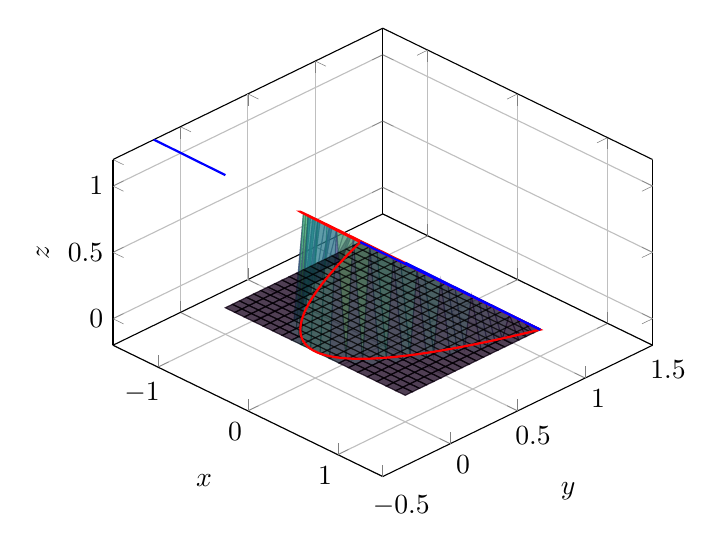
\begin{tikzpicture}
\begin{axis}[
    view={45}{45},
    xlabel=$x$, ylabel=$y$, zlabel=$z$,
    xmin=-1.5, xmax=1.5,
    ymin=-0.5, ymax=1.5,
    zmin=-0.2, zmax=1.2,
    grid=major,
]
    % Use a simple surface for the top part
    \addplot3[surf, domain=-1:1, y domain=0:1, samples=20, opacity=0.5, colormap/viridis] { (y >= x^2) ? (1-y) : 0 };
    
    % Use a simple surface for the bottom part
    \addplot3[surf, domain=-1:1, y domain=0:1, samples=20, opacity=0.5, colormap/gray] { (y >= x^2) ? 0 : 0 };

    % Use parametric plots for the boundaries
    % Bottom boundary: y = x^2, z = 0
    \addplot3[thick, red, domain=-1:1, samples=50] ({x}, {x^2}, {0});
    % Top boundary: y = x^2, z = 1 - x^2
    \addplot3[thick, red, domain=-1:1, samples=50] ({x}, {x^2}, {1-x^2});
    % Back/Side boundaries:
    % y = 1, z = 0 (at x in [-1,1])
    \addplot3[thick, blue, domain=-1:1, samples=50] ({x}, {1}, {0});
    % y = 1, z = 0 (Wait, y+z=1 means if y=1, z=0. Correct.)
    % The plane z = 1-y intersects y=1 at z=0.
    % Let's add the line where the top plane meets the plane y=1.
    % It's the line y=1, z=0.
    
    % Let's add the top edge: y+z=1 and y=1 => z=0.
    % Let's add the top edge: y+z=1 and x=1 => z=1-y.
    \addplot3[thick, blue, domain=0:1, samples=50] ({1}, {y}, {1-y});
    \addplot3[thick, blue, domain=-1:0, samples=50] ({-1}, {y}, {1-y});

\end{axis}
\end{tikzpicture}
\end{document}
